% !TeX root = ../main.tex
\chapter{Differential calculus in higher dimension}

\lettrine{I}{n} this part of the course we start to consider higher dimensional space.
That is, instead of \(\bR\) we consider \(\bR^n\) for \(n\in \bN\).
We will particularly focus on 2D and 3D but everything also holds in any dimension.
Going beyond \(\bR\) we have more options for functions and correspondingly more options for derivatives.

Various different notation is commonly used.
Here we will primarily use \((x,y)\in \bR^2\), \((x,y,z)\in\bR^3\) or, more generally,  \(\xx =(x_1,x_2,\ldots,x_n) \in \bR^n \)
where
\( x_1 \in \mathbb{R},\ldots, x_n \in \mathbb{R}\).
For example, \(\bR^2\) is the plane, \(\bR^3\) is 3D space.

\begin{definition}[inner product]
    \(\xx \cdot \yy = \sum_{k=1}^{n} x_k y_k \in \bR\)
\end{definition}

\noindent
We recall that the inner product being zero has a geometric meaning, it means that the two vectors are orthogonal.
We also recall that the ``length'' of a vector is given by the norm, defined as follows.

\begin{definition}[norm]
    \(\norm{\xx} =  \sqrt{\xx \cdot \xx} = (\sum_{k=1}^{n} x_k^2 )^{\frac{1}{2}}\).
\end{definition}

\noindent
For example, in \(\bR^2\) then \(\norm{(x,y)} = \sqrt{x^2 + y^2}\).
There are various convenient properties for working with norms and inner products, in particular, the \href{https://en.wikipedia.org/wiki/Cauchy%E2%80%93Schwarz_inequality}{Cauchy-Schwarz inequality} \(\abs{x\cdot y} \leq \norm{\xx} \ \norm{\yy}\) and the \href{https://en.wikipedia.org/wiki/Triangle_inequality}{triangle inequality} \(\norm{\xx + \yy} \leq \norm{\xx} + \norm{\yy}\).

\begin{samepage}
    The primary higher-dimensional functions we consider in this course are:
    \begin{center}
        \begin{tabular}{r l}
            Scalar fields:
             &
            \(f:\bR^n \to \bR\)                   \\
            Vector fields:
             &
            \(\mathbf{f}:\bR^n \to \bR^n\)        \\
            Paths:
             &
            \(\boldsymbol{\alpha}:\bR \to \bR^n\) \\
            Change of coordinates:
             &
            \(\xx:\bR^n \to \bR^n\)
        \end{tabular}
    \end{center}
\end{samepage}
\noindent
These possibilities all fit into the general pattern of \(f:\mathbb{R}^n \to \mathbb{R}^m\) for $n,m\in \mathbb{N}$ but tradition and use of the function gives us different terminology and symbols.
Such functions are useful for representing various practical things, for example:
gravitational force; temperature in a region; wind velocity; fluid flow; electric field; etc.



\section{Open sets, closed sets, boundary, continuity}

Let \(\aa \in \bR^n\), \(r>0\).
The open \(n\)-ball of radius \(r\) and centre \(\aa\) is written as
\[
    B(\aa,r):= \left\{ \xx \in \bR^n : \norm{\xx - \aa}< r  \right\}.
\]

\begin{definition}[interior point]
    Let \(S \subset \bR^n\).
    A point \(\aa \in S\) is said to be an \emph{interior point} if there is \(r>0\) such that \( B(\aa,r) \subset S\).
    The set of all interior points of \(S\) is denoted \(\operatorname{int} S\).
\end{definition}

\begin{definition}[open set]
    A set \(S \subset \bR^n\) is said to be \emph{open} if all of its points are interior points, i.e., if \(\operatorname{int} S = S\).
\end{definition}



\begin{figure}[htbp]
    \begin{center}
        \includegraphics{interior.pdf}
        \caption{Interior points are the centre of a ball contained within the set.}
    \end{center}
\end{figure}


For example,
open intervals, open disks, open balls, unions of open intervals, etc., are all open sets.

\begin{lemma*}
    Let $r>0$, $\mathbf{x} \in \mathbb{R}^n$. The set $B(\mathbf{a},r) \subset \mathbb{R}^n$ is open.
\end{lemma*}
\begin{proof}
    Let $\mathbf{b} \in B(\mathbf{a},r)$. It suffices to show that $\mathbf{b}$ is an interior point.
    (1) Let $r_1 = \| \mathbf{b} - \mathbf{a} \| < r$.
    (2) Let $r_2 = (r - r_1)/2$.
    (3) We claim that $B(\mathbf{b},r_2) \subset B(\mathbf{a},r)$:
    In order to see this take any $\mathbf{c} \in B(\mathbf{b},r_2)$ and observe that
    $$\| \mathbf{c} - \mathbf{a} \| \leq \| \mathbf{c} - \mathbf{b} \|  + \| \mathbf{b} - \mathbf{a} \| \leq r_2 + r_1 = \frac{r + r_1}{2} < r.$$
    Observe that the radius of the ball will be small for points close to the boundary.
\end{proof}



\begin{definition}[Cartesian product]
    If \(A_1 \subset \bR\), \(A_2 \subset \bR\) then the \emph{Cartesian product} is defined as
    \[
        A_1 \times A_2 := \left\{(x,y): x \in A_1, y \in A_2\right\}
        \subset \bR^{2}.
    \]
\end{definition}

Analogously the Cartesian product can be defined in higher dimensions:
If \(A_1 \subset \bR^m\), \(A_2 \subset \bR^n\) then the \emph{Cartesian product} \(A_1 \times A_2\) is defined as the set of all points \((x_1,\ldots,x_m,y_1,\ldots,y_n) \in \bR^{m+n}\) such that \((x_1,\ldots,x_m) \in A_1\) and \((y_1,\ldots,y_n) \in A_2\).


\begin{lemma*}
    If \(A_1, A_2\) are open subsets of \(\bR\) then \( A_1 \times A_2 \) is an open subset of \(\bR^2\).
\end{lemma*}
\begin{proof}
    Let \(\aa = (a_1,a_2) \in A_1\times A_2 \subset \bR^2\).
    Since  \(A_1\) is open there  exists \(r_1>0\) such that \(B(a_1,r_1)\subset A_1\).
    Similarly for \(A_2\).
    Let \(r=\min \{r_1,r_2\}\).
    This all means that \(B(\aa,r) \subset B(a_1,r_1) \times B(a_2,r_2) \subset A_1\times A_2\).
\end{proof}


\begin{figure}[htb]
    \begin{centering}
        \includegraphics{cartesian.pdf}
        \caption{If \(A_1, A_2\) are intervals then \( A_1 \times A_2 \) is a rectangle.}
    \end{centering}
\end{figure}

Discussing the ``interior'' of the set naturally suggests the topic of the ``boundary'' of the set.
In the following definitions we develop this idea.


\begin{definition}[exterior points]
    Let \(S\subset \bR^n\).
    A point \(\aa \notin S\) is said to be an \emph{exterior point} if there exists \(r>0\) such that \(B(\aa,r)\cap S = \emptyset\).
    The set of all exterior points of \(S\) is denoted \(\operatorname{ext} S\).
\end{definition}

Observe that \(\operatorname{ext} S\) is an open set.
We use the notation \(S^c = \bR^n \setminus S\) and we say that \(C^c\) is the \emph{complement} of the set \(S\).



\begin{definition}[boundary]
    The set \(\bR^n \setminus (\operatorname{int} S \cup \operatorname{ext} S )\) is called the boundary of \(S \subset \bR^n\) and is denoted \(\partial S\).
\end{definition}


\begin{definition}[closed]
    A set \(S\subset \bR^n\) is said to be \emph{closed} if \(\partial S \subset S\).
\end{definition}

\begin{lemma}
    \(S\) is open \(\Longleftrightarrow \) \(S^c\) is closed.
\end{lemma}
\begin{proof}
    Observe that \(\bR^n =  \operatorname{int} S \cup \partial S \cup \operatorname{ext} S\) (disjointly).
    If \(\xx \in \partial S\) then, for every \(r>0\), \(B(\xx,r) \cap S \neq \emptyset\) and so \(\xx \in \partial(S^c)\).
    Similarly with \(S\) and \(S^c\) swapped and so \(\partial S = \partial(S^c)\).
    If \(S\) is open then \(\operatorname{int} S = S\) and \(S^c = \operatorname{ext} S \cup \partial S =  \operatorname{ext} S \cup \partial (S^c)\) and so \(S^c\) is closed.
    If \(S\) is not open then there exists \(\aa \in \partial S \cap S\). Additionally  \(\aa \in \partial (S^c) \cap S\) hence \(S^c\) is not closed.
\end{proof}


\subsection*{Limits and continuity}

Let \(S\subset \bR^n\) and \(\ff : S \to \bR^m\).
If \(\aa\in \bR^n\), \(\bb\in \bR^m\) we write
    {\(  \displaystyle\lim_{\xx \to \aa}\ff(\xx) = \bb \)}
to mean that
\(\norm{\ff(\xx)-\bb} \to 0\) as \(\norm{\xx-\aa}\to 0\).
Observe how, if \(n=m=1\), this is the familiar notion of continuity for functions on \(\bR\).

\begin{definition}[continuous]
    A function \(\ff\) is said to be \emph{continuous} at \(\aa\) if \(\ff\) is defined at \(\aa\) and
    \(  \displaystyle\lim_{\xx \to \aa}\ff(\xx) = \ff(\aa)\).
    We say \(\ff\) is continuous on \(S\) if \(\ff\) is continuous at each point of \(S\).
\end{definition}

Even functions which look ``nice'' can fail to be continuous as we can see in the following example.

\begin{example*}[continuity in higher dimensions]
    Let \(f(x,y)\) be defined, for \((x,y)\neq (0,0)\), as
    \[
        f(x,y) =
        \frac{x y}{x^2 + y^2}
    \]
    and \(f(0,0)=0\).
    What is the behaviour of \(f\) when approaching \((0,0)\) along the following lines?
    \begin{center}
        \begin{tabular}{ c | c }
            line         & value                     \\
            \hline
            \(\{x=0\}\)  & \(f(0,t) =  0\)           \\
            \(\{y=0\}\)  & \(f(t,0) = 0\)            \\
            \(\{x=y\}\)  & \(f(t,t) = \frac{1}{2}\)  \\
            \(\{x=-y\}\) & \(f(t,t) =-\frac{1}{2}\).
        \end{tabular}
    \end{center}
\end{example*}

\begin{theorem}
    Suppose that \(  \lim_{\xx \to \aa}\ff(\xx) = \bb\) and \(  \lim_{\xx \to \aa}\gg(\xx) = \cc\).
    Then
    \begin{enumerate}
        \item \(  \lim_{\xx \to \aa}(\ff(\xx)+\gg(\xx)) = \bb+\cc\),
        \item \(  \lim_{\xx \to \aa} \lambda \ff(\xx) = \lambda \bb\) for every \(\lambda \in \bR\),
        \item \(  \lim_{\xx \to \aa}\ff(\xx)\cdot \gg(\xx) = \bb\cdot \cc\),
        \item \(  \lim_{\xx \to \aa} \norm{\ff(\xx)} = \norm{\bb}\).
    \end{enumerate}
\end{theorem}

We prove a couple of the parts of the above theorem here, the other parts are left as exercises.

\begin{proof}[Proof of (c)]
    Observe that  \(
    \ff(\xx)\cdot\gg(\xx) - \bb\cdot \cc
    = (\ff(\xx)-\bb)\cdot(\gg(\xx)-\cc) + \bb\cdot(\gg(\xx)-\cc) + \cc\cdot(\ff(\xx)-\bb)
    \).
    By the triangle inequality and Cauchy-Schwarz,
    \[
        \begin{aligned}
            \norm{\ff(\xx)\cdot\gg(\xx) - \bb\cdot \cc }
             & \leq \norm{\ff(\xx)-\bb} \norm{\gg(\xx)-\cc} \\
             & \quad + \norm{\bb}\norm{\gg(\xx)-\cc}        \\
             & \quad + \norm{\cc} \norm{\ff(\xx)-\bb}.
        \end{aligned}
    \]
    Since \(\norm{\ff(\xx)-\bb} \to 0\) and \(\norm{\gg(\xx)-\cc} \to 0\) as \(\xx \to \aa\) this implies that \(\norm{\ff(\xx)\cdot\gg(\xx) - \bb\cdot \cc }\to 0\).
\end{proof}

\begin{proof}[Proof of (d)]
    Take \(\ff = \gg\) in part (c) implies that \(   \lim_{\xx \to \aa} \norm{\ff(\xx)}^2 = \norm{\bb}^2\).
\end{proof}


When writing a vector field (or similar functions) it is often convenient to divide the higher-dimensional function into smaller parts.
We call these parts the \emph{components of a vector field}.
For example \(\ff(\xx) = \left(f_1(\xx),f_2(\xx)\right)\) in 2D, \(\ff(\xx) = \left(f_1(\xx),f_2(\xx),f_3(\xx)\right)\) in 3D, etc.

\begin{theorem}
    Let \(\ff(\xx) = \left(f_1(\xx),f_2(\xx)\right)\).
    Then \(\ff\) is continuous if and only if \(f_1\) and \(f_2\) are continuous.
\end{theorem}
\begin{proof}
    We will independently prove the two implications.
    \begin{description}
        \item[(\(\Rightarrow\))]
            Let
            \( \ee_1=(1,0) \), \( \ee_2=(0,1) \)
            and observe that \(f_k(\xx) = \ff(\xx)\cdot \ee_k\).
            We have already shown that the continuity of two vector fields implies the continuity of the inner product.
        \item[(\(\Leftarrow \))]
            By definition of the norm
            \(\norm{\ff(\xx)-\ff(\aa)}^2 = \displaystyle\sum_{k=1}^{2}(f_k(\xx)-f_k(\aa))^2\)
            and we know \(\norm{f_k(\xx)-f_k(\aa)} \to 0\) as \(\norm{\xx-\aa}\to 0\). \qedhere
    \end{description}
\end{proof}

In higher dimensions the analogous statement is true for the vector field \(\ff(\xx) = \left(f_1(\xx),\ldots,f_m(\xx) \right)\) with exactly the same proof.
I.e., \(\ff\) is continuous if and only if each \(f_k\) is continuous.


\begin{example*}[polynomials]
    A  \emph{polynomial} in \(n\) variables is a scalar field on \(\bR^n\) of the form
    \[
        f(x_1,\ldots,x_n)
        = \sum_{k_1=0}^{j}\cdots \sum_{k_n=0}^{j} c_{k_1,\dots,k_n} x_1^{k_1}\cdots x_n^{k_n}.
    \]
    E.g., \(f(x,y):= x + 2x y - x^2\) is a polynomial in \(2\) variables.
    Polynomials are continuous everywhere in \(\bR^n\). This is because they are the finite sum of products of continuous scalar fields.
\end{example*}

\begin{example*}[rational functions]
    A  \emph{rational function} is a scalar field
    \[
        f(\xx)=\frac{p(\xx)}{q(\xx)}
    \]
    where \(p(\xx)\) and \(q(\xx)\) are polynomials.
    A rational function is continuous at every point \(\xx\) such that \(q(\xx)\neq 0\).
\end{example*}

As described in the following result, the continuity of functions continues to hold, in an intuitive way, under composition of functions.

\begin{theorem}
    Suppose \(S \subset \bR^l\), \(T\subset \bR^m\), \(\ff:S \to \bR^m\), \(\gg : T \to \bR^n\) and that \(\ff(S) \subset T\) so that
    \[(\gg \circ \ff)(\xx) = \gg(\ff(\xx))\]
    makes sense.
    If \(\ff\) is continuous at \(\aa\in S\) and \(\gg\) is continuous at \(\ff(\aa)\) then \(\gg\circ \ff\) is continuous at \(\aa\).
\end{theorem}

\begin{proof}
    \(\displaystyle\lim_{\xx\to\aa}\norm{\ff(\gg(\xx))-\ff(\gg(\aa))}  =\displaystyle\lim_{\yy\to\gg(\aa)}\norm{\ff(\yy)-\ff(\gg(\aa))}  =0   \)
\end{proof}

\begin{example*}
    We can consider the scalar field \(f(x,y)= \sin(x^2 + y) + x y\) as the composition of functions.
\end{example*}


\section{Derivatives of scalar fields}

\begin{figure}
    \begin{center}
        \includegraphics[width=0.5\textwidth]{gradient.pdf}
        \caption{Plot where colour represents the value of \(f(x,y)=x^2 + y^2\). The change in \(f\) depends on direction.}
        \label{fig:directional}
    \end{center}
\end{figure}

We can imagine, for example in Figure~\ref{fig:directional}, that in higher dimensions, the derivative of a scalar field depends on the direction.
This motivates the following.

\begin{definition}[directional derivative]
    Let \(S\subset \bR^n\) and \(f:S\to \bR\).
    For any \(\aa \in \operatorname{int}S\) and \(\vv \in \bR^n\), \(\norm{v}=1\) the directional derivative of \(f\) with respect to \(\vv\) is defined as
    \[
        D_{\vv}f(\aa) =
        \lim_{h\to 0} \frac{1}{h}\left(  f(\aa+h \vv) - f(\aa)     \right).
    \]
\end{definition}


When \(h\) is small we can guarantee that \(\aa + h \vv \in S\) because \(\aa\in \operatorname{int} S\) so this definition makes sense.


\begin{theorem*}
    Suppose \(S\subset \bR^n\), \(f:S\to \bR\), \(\aa \in \operatorname{int} S\).
    Let \(g(t) := f(\aa + t\vv)\).
    If one of the derivatives \(g'(t)\) or \(D_\vv f(\aa)\) exists then the other also exists and
    \[
        g'(t) = D_{\vv}f(\aa+t \vv).
    \]
    In particular \(g'(0) = D_{\vv}f(\aa)\).
\end{theorem*}

\begin{proof}
    By definition \(\frac{1}{h}(g(t+h)-g(h)) =\frac{1}{h}(f(\aa+h \vv) - f(\aa)) \).
\end{proof}

The following result is useful for proving later results.

\begin{theorem*}[mean value]
    Assume that \(D_{\vv}(\aa+t\vv)\)  exists for each \(t\in [0,1]\). Then for some \(\theta \in (0,1)\),
    \[
        f(\aa+\vv) - f(\aa) = D_{\vv}f (\zz),
        \quad
        \text{where \(z=\aa + \theta \vv\)}.
    \]
\end{theorem*}

\begin{proof}
    Apply mean value theorem to \(g(t) = f(\aa+t\vv)\).
\end{proof}


The following notation is convenient.
For any \(k\in\{1,2,\ldots,n\}\),
let \(\ee_k\) be the \(n\)-dimensional unit vector where all entries are zero except the \(k\)\textsuperscript{th} position which is equal to \(1\).
I.e., \( \ee_1=(1,0,\ldots,0)  \),  \( \ee_1=(0,1,0,\ldots,0)  \),  \( \ee_1=(0,\ldots,0,1)  \).

\begin{definition}[partial derivatives]
    We define the \emph{partial derivative} in \(x_k\) of \(f(x_1,\ldots,x_n)\) at \(\aa\) as
    \[
        \frac{\partial f}{\partial x_k}(\aa) = D_{\ee_k}f(\aa).
    \]
\end{definition}


\begin{remark*}
    Various symbols used for partial derivatives:
    \(\frac{\partial f}{\partial x_k}(\aa) = D_kf(\aa) = \partial_{k}f(\aa)\).
    If  a function is written \(f(x,y)\) we write \(\frac{\partial f}{\partial x}, \frac{\partial f}{\partial y}\) for the partial derivatives. Similarly for higher dimension.
\end{remark*}

In practice, to compute the partial derivative \( \frac{\partial f}{\partial x_k}\), one should consider all other \(x_j\) for \(j\neq k\) as constants and take the derivative with respect to \(x_k\).
In a moment we see this rigorously.


If \(f:\bR \to \bR\) is differentiable, then we know that, when \(x\) is close to \(a\),
\[
    f(x) \approx f(a) + (x-a) f'(a).
\]
More precisely, we know that\footnote{This is \href{https://en.wikipedia.org/wiki/Big_O_notation\#Little-o_notation}{\emph{little-o notation}} and here means that \(\abs{f(x) - f(a) - (x-a) f'(a)}/\abs{x-a} \to 0\) as \(\abs{x-a}\to 0\).  } \(f(x) = f(a) + (x-a) f'(a) + \epsilon(x-a)\) where \(\abs{\epsilon(x-a)} = \littleo{\abs{x-a}}\).
This way of seeing differentiability is convenient for the higher dimensional definition of differentiability.

\begin{definition*}[differentiable]
    Let \(S\subset \bR^n\) be open, \(f:S \to \bR\).
    We say that \(f\) is \emph{differentiable} at \(\aa \in S\) if there exists a linear transformation \({df}_{\aa}: \bR^n \to \bR\) such that, for \(\xx \in B(\aa,r)\),
    \[
        f(\xx) = f(\aa) + {df}_{\aa}(\xx-\aa) + \epsilon(\xx-\aa)
    \]
    where \(\abs{\epsilon(\xx-\aa)} = \littleo{\norm{\xx-\aa}}\).
\end{definition*}


For future convenience we introduce the following notation.
%
\begin{definition}[gradient]
    The \emph{gradient} of the scalar field \(f(x,y,z)\) at the point \(\aa\) is
    \[
        \nabla f(\aa) =
        \begin{pmatrix}
            \frac{\partial f}{\partial x}(\aa) \\[2pt]
            \frac{\partial f}{\partial y}(\aa) \\[2pt]
            \frac{\partial f}{\partial z}(\aa)
        \end{pmatrix}.
    \]
\end{definition}
%
\noindent
In general, when working in \(\bR^n\) for some \(n\in\bN\), the \emph{gradient} of the scalar field \(f(x_1,\ldots,x_n)\) at the point \(\aa\) is
\[
    \nabla f(\aa) =
    \begin{pmatrix}
        \frac{\partial f}{\partial x_1}(\aa) \\[2pt]
        \frac{\partial f}{\partial x_2}(\aa) \\[2pt]
        \vdots                               \\
        \frac{\partial f}{\partial x_n}(\aa)
    \end{pmatrix}.
\]


\begin{theorem}
    \label{thm:differential}
    If \(f\) is differentiable at \(\aa\)
    then \({df}_{\aa}(\vv) = \nabla f(\aa) \cdot \vv \).
    This means that, for \(\xx \in B(\aa,r)\),
    \[
        f(\xx) = f(\aa) +   \nabla f(\aa) \cdot (\xx-\aa) + \epsilon(\xx-\aa)
    \]
    where \(\abs{\epsilon(\xx-\aa)} = \littleo{\norm{\xx-\aa}}\).
    Moreover, for any vector \(\vv\), \(\norm{v}=1\),
    \[
        D_{\vv}f(\aa) = \nabla f(\aa) \cdot \vv.
    \]
\end{theorem}

\begin{proof}
    Since \(f\) is differentiable there exists a linear transformation \({df}_{\aa}: \bR^n \to \bR\) such that
    \(  f(\aa+ h \vv) = f(\aa) + h {df}_{\aa}(\vv) + \epsilon(h\vv)\)
    and hence
    \[
        \begin{aligned}
            D_{\vv}f(\aa) & =
            \lim_{h\to 0} \frac{1}{h}(f(\aa+h \vv) - f(\aa)) \\
                          & =
            \lim_{h\to 0} \frac{1}{h}(h \ {df}_{\aa}(\vv) + \epsilon(h\vv) )
            =  {df}_{\aa}(\vv).
        \end{aligned}
    \]
    In particular \({df}_{\aa}(\ee_k) = D_{\ee_k}f(\aa)\).
\end{proof}


\begin{theorem*}
    If \(f\) is differentiable at \(\aa\), then it is continuous at \(\aa\).
\end{theorem*}
\begin{proof}
    Observe that \(\abs{f(\aa+\vv)-f(\aa)} = \abs{   {df}_{\aa}(\vv) + \epsilon(\vv)  }\).
    Consequently \( \abs{f(\aa+\vv)-f(\aa)} \leq \norm{  {df}_{\aa} } \norm{\vv} + \abs{\epsilon(\vv)} \) and this tends to \(0\) as \(\norm{\vv} \to 0\).
\end{proof}

\begin{theorem}
    Suppose that \(f(x_1,\ldots,x_n)\) is a scalar field.
    If the partial derivatives \(\partial_1 f(\xx), \ldots, \partial_nf(\xx)\) exist for all \(\xx\in B(\aa,r)\) and are continuous at \(\aa\) then \(f\) is differentiable at \(\aa\).
\end{theorem}

\begin{proof}
    For convenience write \(\vv = (v_1,v_2,\ldots,v_n)\)     and     \(\uu_k = (v_1,v_2,\ldots,v_k,0,\ldots,0)\).
    \begin{enumerate}
        \item Observe that \(\uu_k - \uu_{k-1} = v_k \ee_k\), \(\uu_0 = (0,0,\ldots,0)\) and \(\uu_n = \vv\);
        \item Using the mean value theorem (exists \( \zz_k = \uu_{k-1}+ \theta_k \ee_k\)) \vspace{-0.9em}
              \[
                  \begin{aligned}
                      f(\aa+\vv) - f(\aa)
                       & = \sum_{k=1}^{n} f(\aa + \uu_k) - f(\aa + \uu_{k-1})
                      = \sum_{k=1}^{n} v_k  D_{\ee_k}f(\aa +  \zz_k)                                                                  \\
                       & = \sum_{k=1}^{n} v_k  D_{\ee_k}f(\aa + \uu_{k-1})                                                            \\
                       & \ \ \ \ \ \ \ \ + \sum_{k=1}^{n}  v_k \left(  D_{\ee_k}f(\aa +  \zz_k)-  D_{\ee_k}f(\aa + \uu_{k-1}) \right)
                  \end{aligned}
              \]
        \item \(\sum_{k=1}^{n} v_k  D_{\ee_k}f(\aa + \uu_{k-1}) \to \vv \cdot \nabla f(\aa)\). \qedhere
    \end{enumerate}
\end{proof}


\subsection*{Chain rule}

When we are working in \(\bR\) we know that, if \(g\) and \(h\) are differentiable, then \(f(t) = g\circ h(t)\) is also differentiable and also \(f'(t) = g'(h(t)) \ h'(t)\).
This is called the \emph{chain rule} and is frequently very useful in calculating derivatives.
We now investigate how this extends to higher dimension?

\begin{example*}
    Suppose that
    \begin{itemize}
        \item \(\aalpha:\bR \to \bR^3\) describes the position \(\aalpha(t)\) at time \(t\),
        \item \(f:\bR^3 \to \bR\) describes the temperature \(f(\aalpha)\) at a point \(\aalpha\)
    \end{itemize}
    The temperature at time \(t\) is equal to \(g(t)=f(\aalpha(t))\).
    We want to calculate \(g'(t)\) because this is the change in temperature with respect to time.
\end{example*}

Consequently it is convenient to consider the derivative of a path \(\aalpha:\bR \to \bR^n\).
Let \(\aalpha:\bR \to \bR^n\) and suppose it has the form
\(\aalpha(t) = \left( \alpha_1(t), \ldots, \alpha_n(t)  \right)\).
We define the derivative as
\[
    \aalpha'(t) := \begin{pmatrix}
        x_1'(t) \\
        \vdots  \\
        x_n'(t)
    \end{pmatrix}.
\]
\noindent
Here \(\aalpha'\) is a vector-valued function which represents the ``direction of movement''.

\begin{figure}[htb]
    \begin{center}
        \includegraphics[width=0.5\textwidth]{spiral.pdf}
        \caption{\(\aalpha(t)=(\cos t, \sin t, t)\), \(t\in \bR\).}
        \label{fig:spiral}
    \end{center}
\end{figure}


\begin{theorem*}
    Let \(S\subset \bR^n\) be open and \(I\subset \bR\) an interval.
    Let \(\xx: I \to S\) and \(f:S \to \bR\) and define, for \(t\in I\),
    \[
        g(t) = f (\xx(t)).
    \]
    Suppose that  \(t\in I\) is such that \(\xx'(t)\) exists and \(f\) is differentiable at \(\xx(t)\).
    Then \(g'(t)\) exists and
    \[
        g'(t) = \nabla f \left(\xx(t)\right) \cdot \xx'(t).
    \]
\end{theorem*}


\begin{proof}
    Let \(h>0\) be small, \vspace{-.5em}
    \[
        \begin{aligned}
            \tfrac{1}{h}\left[g(t+h)-g(t) \right]
             & = \tfrac{1}{h}\left[f(\xx(t+h)-f(\xx(t)))\right]                        \\
             & = \tfrac{1}{h} \nabla f(\xx(t))\cdot (\xx(t+h)-\xx(t))                  \\
             & \ \ +  \tfrac{1}{h}  \norm{\xx(t+h)-\xx(t)} E(\xx(t), \xx(t+h)-\xx(t)).
        \end{aligned}
    \]
    Observe that \(\tfrac{1}{h}  (\xx(t+h)-\xx(t)) \to \xx'(t)  \) as \(h\to 0\).
\end{proof}


\begin{example*}
    A particle moves in a circle and its position at time \(t\in [0,2\pi]\) is given by
    \[
        \xx(t) = (\cos t, \sin t).
    \]
    The temperature at a point \(\yy=(y_1,y_2)\) is given by the function \(f(\yy) := y_1 + y_2\),
    The temperature the particle experiences at time \(t\) is given by \(g(t) = f (\xx(t))\).
    Temperature change:
    \(
    g'(t)
    = \nabla f \left(\xx(t)\right) \cdot \xx'(t)
    = \left(\begin{smallmatrix}
            1 \\
            1
        \end{smallmatrix}\right)
    \cdot
    \left( \begin{smallmatrix}
            -\sin t \\
            \cos t
        \end{smallmatrix}\right)
    = \cos t - \sin t.
    \)
\end{example*}

\begin{figure}
    \begin{center}
        \includegraphics[width=0.5\textwidth]{particle-circle.pdf}
        \caption{\(\xx(t)\) is the position of a particle. Shading represents temperature \(f\).}
        \label{fig:particle-circle}
    \end{center}
\end{figure}


\section{Level sets \& tangent planes}

Let \(S\subset \bR^2\), \(f:S\to\bR\).
Suppose \(c\in \bR\) and let
\[
    L(c) = \left\{\xx\in S : f(\xx)=c\right\}.
\]
The set \(L(c)\) is called the \emph{level set}.
In general this set can be empty or it can be all of \(S\).
However the set \(L(c)\) is often a curve and this is the case of interest.
This is the same notion as that of \href{https://en.wikipedia.org/wiki/Contour_line}{contour lines} on a map.
I.e., \(\xx(t_a) = \aa\) for some \(t_a \in I\) and \[f(\xx(t))=c\] for all \(t\in I\).
Then
\begin{itemize}
    \item \(\nabla f(\aa)\) is normal to the curve at \(\aa\)
    \item Tangent line at \(\aa\) is
          \(\left\{\xx\in\bR^2: \nabla f(\aa) \cdot (\xx-\aa)=0\right\}\)
\end{itemize}

This is because the chain rule implies that \(\nabla f(\xx(t)) \cdot \xx'(t) = 0\).
\begin{example*}
    Let \(f(x_1,x_2,x_3):=x_1^2 + x_2^2 + x_3^2\).
    \begin{itemize}
        \item If \(c>0\) then \(L(c)\) %\(L(c) = \left\{(x_1,x_2,x_3):  x_1^2 + x_2^2 + x_3^2 = c\right\}\)
              is a sphere,
        \item \(L(0) \) is a single point \((0,0,0)\),
        \item If \(c<0\) then \(L(c)\) is empty.
    \end{itemize}
\end{example*}

\begin{example*}
    Let \(f(x_1,x_2,x_3):=x_1^2 + x_2^2 - x_3^2\).
    See Figure~\ref{fig:level-sets}.
    \begin{itemize}
        \item If \(c>0\) then \(L(c)\) is a one-sheeted hyperboloid,
        \item \(L(0) \) is an infinite cone,
        \item If \(c<0\) then \(L(c)\) is a two-sheeted hyperboloid.
    \end{itemize}
\end{example*}

% %                       
\begin{figure}[htb]
    \begin{center}
        \begin{subfigure}[b]{0.24\textwidth}
            \centering
            \includegraphics[width=\textwidth]{sphere.pdf}
            \caption{Sphere}
            \label{fig:sphere}
        \end{subfigure}
        \hfill
        \begin{subfigure}[b]{0.24\textwidth}
            \centering
            \includegraphics[width=\textwidth]{two-hyperboloid.pdf}
            \caption{Two-sheeted hyperboloid}
            \label{fig:two-hyperboloid}
        \end{subfigure}
        \hfill
        \begin{subfigure}[b]{0.24\textwidth}
            \centering
            \includegraphics[width=\textwidth]{infinite-cone.pdf}
            \caption{Infinite cone}
            \label{fig:infinite-cone}
        \end{subfigure}
        \hfill
        \begin{subfigure}[b]{0.24\textwidth}
            \centering
            \includegraphics[width=\textwidth]{one-hyperboloid.pdf}
            \caption{One-sheeted hyperboloid}
            \label{fig:one-hyperboloid}
        \end{subfigure}
        \caption{Various surfaces as level sets.}
        \label{fig:level-sets}
    \end{center}
\end{figure}


Let \(f\) be a differentiable scalar field on \(S\subset \bR^3\) and suppose that \(L(c) = \left\{\xx\in S : f(\xx)=c\right\}\) is a surface.

\begin{itemize}
    \item \(\nabla f(\aa)\) is normal to every curve \(\aalpha(t)\) in the surface which passes through \(\aa\),
    \item Tangent plane at \(\aa\) is
          \(\left\{\xx\in\bR^3: \nabla f(\aa) \cdot (\xx-\aa)=0\right\}\).
\end{itemize}

Same argument as in \(\bR^2\) works in \(\bR^n\).


\begin{figure}
    \centering
    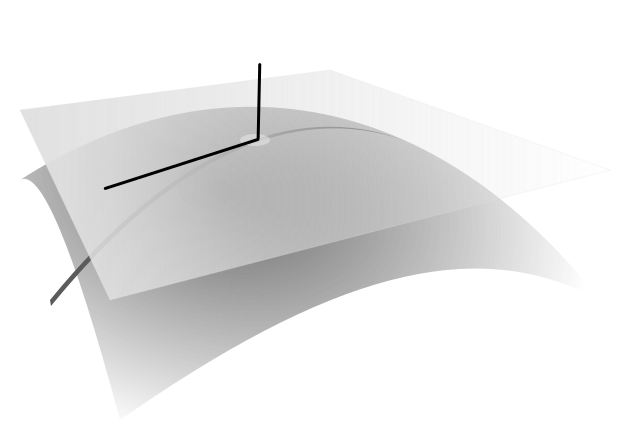
\includegraphics[width=0.8\textwidth]{tangent.pdf}
    \caption{Tangent plane and normal vector}
\end{figure}


\section{Derivatives of vector fields}

Essentially everything discussed above for scalar fields extends to vector fields in a predictable way.
This is because of the linearity and that we can consider each \emph{component} of the vector field independently.

\begin{definition}[directional derivative]
    Let \(S\subset \bR^n\) and \(\ff:S\to \bR^m\).
    For any \(\aa \in \operatorname{int}S\) and \(\vv \in \bR^n\) the derivative of the vector field \(\ff\) with respect to \(\vv\) is defined as
    \[
        D_{\vv}\ff(\aa) :=
        \lim_{h\to 0} \frac{1}{h} \left(\ff(\aa+h \vv) - \ff(\aa)\right).
    \]
\end{definition}

\begin{remark}
    If we write \(\ff = (f_1,\ldots,f_m)\) then \(D_{\vv}\ff = (D_{\vv}f_1,\ldots,D_{\vv} f_m)\).
\end{remark}


\begin{definition*}[differentiable]
    We say that \(\ff: \bR^n \to \bR^m\) is \emph{differentiable} at \(\aa\) if there exists a linear transformation \({df}_{\aa}: \bR^n \to \bR^m\) such that, for \(\xx \in B(\aa,r)\),
    \[
        \ff(\xx) = \ff(\aa) + {df}_{\aa}(\xx-\aa) + \epsilon(\xx-\aa)
    \]
    \(\abs{\epsilon(\xx-\aa)} = \littleo{\norm{\xx-\aa}}\).
\end{definition*}


\begin{theorem}
    If \(\ff\) is differentiable at \(\aa\)
    then \(\ff\) is continuous at \(\aa\)
    and \( {df}_{\aa}(\vv) =D_{\vv}\ff(\aa) \).
\end{theorem}

\begin{proof}
    Same as for the case of scalar fields when \(f:\bR^n \to \bR\).
\end{proof}


\section{Jacobian matrix and chain rule}

The relevant differential for higher-dimensional functions is the \href{https://en.wikipedia.org/wiki/Jacobian_matrix_and_determinant}{Jacobian matrix}.

\begin{definition}[Jacobian matrix]
    Suppose that \(\ff: \bR^2 \to \bR^2\) and use the notation \(\ff(x,y) = (f_1(x,y),f_2(x,y))\).
    The \emph{Jacobian matrix} of \(\ff\) at \(\aa\) is defined as
    \[
        D\ff(\aa) =
        \begin{pmatrix}
            \frac{\partial f_1}{\partial x} (\aa) & \frac{\partial f_1}{\partial y} (\aa) \\[2pt]
            \frac{\partial f_2}{\partial x} (\aa) & \frac{\partial f_2}{\partial y} (\aa)
        \end{pmatrix}.
    \]
\end{definition}

\begin{remark*}
    The \emph{Jacobian matrix} is defined analogously in any dimension.
    I.e., if \(\ff : \bR^n \to \bR^m\) the the Jacobian at \(\aa\) is
    \[
        D\ff(\aa) =
        \begin{pmatrix}
            \partial_1 f_1 (\aa) & \partial_2 f_1 (\aa) & \cdots & \partial_n f_1 (\aa) \\
            \partial_1 f_2 (\aa) & \partial_2 f_2 (\aa) & \cdots & \partial_n f_2 (\aa) \\
            \vdots               & \vdots               &        & \vdots               \\
            \partial_1 f_m (\aa) & \partial_2 f_m (\aa) & \cdots & \partial_n f_m (\aa)
        \end{pmatrix}
    \]
\end{remark*}


If we choose a basis then any linear transformation \(\bR^n \to \bR^m\) can be written as a \(m \times n\) matrix.
We find that \( {df}_{\aa}(\vv ) = D\ff(\aa) \vv\).

Let \(S\subset \bR^n\) and \(\ff : S \to \bR^m\).
If \(f\) is differentiable at \(\aa \in S\) then, for all  \(\xx\in B(\aa,r) \subset S\),
\[
    \ff(\xx) = \ff(\aa) +  D\ff(\aa) (\xx-\aa) + \epsilon(\xx-\aa)
\]
where \(\abs{\epsilon(\xx-\aa)} = \littleo{\norm{\xx-\aa}}\).
This is like a Taylor expansion in higher dimensions.

Here we see that in higher dimensions we have a matrix form of the chain rule.

\begin{theorem}
    \label{thm:jacobian-chain}
    Let \(S\subset \bR^l\), \(T\subset \bR^m\) be open.
    Let \(\ff: S \to T\) and \(\gg:T \to \bR^n\) and define
    \[
        \hh := \gg \circ \ff : S \to \bR^n.
    \]
    Let  \(\aa\in S\). Suppose that \(\ff\) is differentiable at \(\aa\) and \(\gg\) is differentiable at \(\ff(\aa)\).
    Then \(\hh\) is differentiable at \(\aa\) and
    \[
        D\hh(\aa) = D\gg(\ff(\aa)) \ D\ff(\aa).
    \]
\end{theorem}

\begin{proof}
    Let \(\uu = \ff(\aa+\vv) - \ff(\aa) \).
    Since \(\ff\) and \(\gg\) are differentiable,
    \[
        \begin{aligned}
            \hh(\aa+\vv) - \hh(\aa)
             & = \gg(\ff(\aa+\vv)) - \gg(\ff(\aa))                                                                                    \\
             & = D\gg(\ff(\aa))(\ff(\aa+\vv) - \ff(\aa) ) + \boldsymbol{\epsilon}_{\gg}(\uu)                                          \\
             & = D\gg(\ff(\aa))   D\ff(\aa) \vv + D\gg(\ff(\aa))\boldsymbol{\epsilon}_{\ff}(\vv)  + \boldsymbol{\epsilon}_{\gg}(\uu).
        \end{aligned} \qedhere
    \]
\end{proof}



\begin{example}[polar coordinates]
    Here we consider \emph{polar coordinates} and calculate the Jacobian of this transformation.
    We can write the change of coordinates
    \[
        (r,\theta) \mapsto (r\cos \theta, r\sin \theta)
    \]
    as the function  \(\ff(r,\theta) = (x(r,\theta),y(r,\theta))\) where \(\ff:(0,\infty)\times [0,2\pi) \to \bR^2\).
    We calculate the Jacobian matrix of this transformation
    \[
        D\ff(r,\theta) =
        \begin{pmatrix}
            \partial_{r}x(r,\theta) & \partial_{\theta}x(r,\theta) \\
            \partial_{r}y(r,\theta) & \partial_{\theta}y(r,\theta)
        \end{pmatrix}
        =
        \begin{pmatrix}
            \cos \theta & -r\sin \theta \\
            \sin \theta & r\cos \theta
        \end{pmatrix}.
    \]
    In particular we see that \(\det D\ff(r,\theta) = r\), the familiar value used in change of variables with polar coordinated.

    Suppose now that we wish to calculate derivatives of \(h := g \circ \ff\) for some  \(g:\bR^2 \to \bR\).
    \[
        \begin{aligned}
            Dh(r,\theta) & = Dg(\ff(r,\theta)) \ D\ff(r,\theta) \\
            \begin{pmatrix}
                \partial_r h(r,\theta) & \partial_\theta h(r,\theta)
            \end{pmatrix}
                         & =
            \begin{pmatrix}
                \partial_x g(\ff(r,\theta)) & \partial_y g(\ff(r,\theta))
            \end{pmatrix}
            \begin{pmatrix}
                \cos \theta & -r\sin \theta \\
                \sin \theta & r\cos \theta
            \end{pmatrix}
        \end{aligned}
    \]
    In other words
    \[
        \begin{cases}
            \partial_r h(r,\theta) = \partial_x g(r\cos \theta, r\sin \theta) \cos \theta + \partial_y g(r\cos \theta, r\sin \theta)\sin \theta \\
            \partial_\theta h(r,\theta) = - r \partial_x g(r\cos \theta, r\sin \theta) \sin \theta +  r \partial_y g(r\cos \theta, r\sin \theta)\cos \theta
        \end{cases}.
    \]
\end{example}






\section{Implicit functions and partial derivatives}

Just like with derivatives, we can take higher order partial derivatives.
\begin{remark*}
    For convenience when we want to write \(\frac{\partial}{\partial y}\frac{\partial}{\partial x}f(x,y) \), i.e., differentiate first with respect to \(x\) and then with respect to \(y\), we write instead \(\frac{\partial^2 f}{\partial y \partial x}(x,y) \).
    The analogous notation is used for higher derivatives and any other choice of coordinates.
\end{remark*}

We first consider the question of when
\[
    \frac{\partial^2 f}{\partial y \partial x}(x,y)
    \overset{\text{\large\color{blue} ?}}{=}
    \frac{\partial^2 f}{\partial x \partial y}(x,y).
\]

\begin{example*}[partial derivative problem]
    Let \(f:\bR^2 \to \bR\) be defined as \(f(0,0)=0\) and, for \((x,y)\neq (0,0)\),
    \[
        f(x,y) := \frac{x y(x^2 - y^2)}{x^2 + y^2}.
    \]
    We calculate that \(\frac{\partial^2 f}{\partial y \partial x} (0,0) = -1\) but
    \(\frac{\partial^2 f}{\partial x \partial y}(0,0) = 1\).
\end{example*}

\begin{theorem}
    Let \(f:S\to\bR\) be a scalar field such that the partial derivatives \(\frac{\partial f}{\partial x }\), \(\frac{\partial f}{\partial y}\) and \(\frac{\partial^2 f}{\partial y \partial x} \) exist on an open set \(S\subset \bR^2\) containing \(\xx\).
    Further assume that \(\frac{\partial^2 f}{\partial y \partial x} \) is continuous on \(S\).
    Then the derivative \(\frac{\partial^2 f}{\partial x \partial y} (\xx)\) exists and
    \[
        \frac{\partial^2 f}{\partial x \partial y} (\xx)=\frac{\partial^2 f}{\partial y \partial x}  f(\xx).
    \]
\end{theorem}

In many cases we can choose to write a given curve/function either in \emph{implicit} or \emph{explicit} form.

\begin{center}
    \begin{tabular}{c | c}
        \textbf{Implicit}         & \textbf{Explicit}                              \\
        \hline
        \(x^2-y=0\)               & \(y(x) = x^2\)                                 \\
        \(x^2+y^2=1\)             & \(y(x) = \pm \sqrt{1-x^2}\), \(\abs{x}\leq 1\) \\
        \(x^2-y^2-1=0\)           & \(y(x) = \pm \sqrt{x^2-1}\), \(\abs{x}\geq 1\) \\
        \(x^2+y^2-e^y -4 =0\)     & A mess?                                        \\
        \(x^2y^4 - 3 = \sin(xy)\) & A huge mess?
    \end{tabular}
\end{center}

Given the above observation, the following method of calculating derivatives is sometimes useful.
Suppose that some \(f:\bR^2 \to \bR\) is given and we suppose there exists some \(y:\bR\to\bR\) such that
\[
    f(x,y(x))=0 \quad \text{ for all \(x\)}.
\]
Let \(h(x):= f(x,y(x))\) and note that \(h'(x)=0\).
Here we are using the idea that \(h = f \circ g\) where \(g(x) = (x,y(x))\).
By the chain rule \( h'(x)\) is equal to
\[
    \begin{pmatrix}
        \frac{\partial f}{\partial x}(x,y(x)) & \frac{\partial f}{\partial y}(x,y(x))
    \end{pmatrix}
    \begin{pmatrix}
        1 \\
        y'(x)
    \end{pmatrix}
    =0.
\]
Consequently
\[
    y'(x) = - \frac{ \frac{\partial f}{\partial x}(x,y(x)) }{ \frac{\partial f}{\partial y}(x,y(x)) }.
\]
